\documentclass[12pt, oneside]{report}\usepackage[]{graphicx}\usepackage[]{color}
% maxwidth is the original width if it is less than linewidth
% otherwise use linewidth (to make sure the graphics do not exceed the margin)
\makeatletter
\def\maxwidth{ %
  \ifdim\Gin@nat@width>\linewidth
    \linewidth
  \else
    \Gin@nat@width
  \fi
}
\makeatother

\usepackage{Sweavel}


\usepackage[margin=0.85in]{geometry}
\linespread{1}
\usepackage{xcolor}
\usepackage[colorlinks=false, linkbordercolor=white, citebordercolor=white, 
    filebordercolor=white, urlbordercolor=white]{hyperref}
    
\usepackage{graphicx}
\usepackage[utf8]{inputenc}
\usepackage[english]{babel}
\usepackage[T1]{fontenc}

\usepackage{fancyhdr}
\pagestyle{fancy}
\renewcommand{\headrulewidth}{0.4pt}
\fancyhead{}
\fancyhead[L]{Statistics for Computer Science -- assignment 1} %%% change to your course name and change the number accordingly
\fancyhead[R]{Martin Gregorík} %%% change to your first name and surname
\fancyfoot{}
\fancyfoot[C]{\thepage}

\usepackage{titlesec}
\titlespacing{\chapter}{0pt}{*4}{*2.5}

\titleformat{\chapter}{\normalfont\huge\bf}{\thechapter}{20pt}{\huge\bf}


% Setting up of environment
\usepackage{listings}
\definecolor{dgray}{gray}{0.35} % colour of comments
\definecolor{lgray}{gray}{0.95} % background colour of R-code
\definecolor{llgray}{gray}{0.98} % background colour of R-outputs

\lstdefinestyle{Rstyle}{ % settings of R-code style
language=R, % setting language R
basicstyle=\ttfamily\small, % font and size of R-code
backgroundcolor=\color{lgray}, % background colour of R-code
commentstyle=\ttfamily\small\itshape\color{dgray}, % colour of R comments
showstringspaces=false, % forbidding the highlighting of spaces
numbers=left, % numbering on the left
numberstyle=\ttfamily\small, % font and size of numbering
stepnumber=1, % numbering with step 1
firstnumber=last, % cumulative numbering of rows in consecutive Chunks
breaklines=T} % automatic line breaks of code at the end of a line

\lstdefinestyle{Routstyle}{ %  settings of R-output style
language=R, % setting language R
basicstyle=\ttfamily\small, % font and size of R-output
backgroundcolor=\color{llgray}, % background colour of R-code
showstringspaces=false, % forbidding the highlighting of spaces
numbers=right, % numbering on the right
numberstyle=\ttfamily\small, % font and size of numbering
firstnumber=last, % cumulative numbering of rows in consecutive Chunks
breaklines=T} % automatic line breaks of code at the end of a line

\begin{document}



\begin{titlepage}
    \begin{center}
        \vspace*{1cm}
        
        \Huge
          \textbf{Statistics for Computer Science} %%% change to your course name
        
        \vspace{0.5cm}
        \LARGE
        Assignment 1 %%% change the number accordingly
        
        \vspace{1.5cm}
        
        \textbf{Martin Gregorík} %%% change to your first name and surname
   		  \vspace{1.5cm}
        
        \textbf{500359} %%% change to your UCO
       
        \vfill
        
        Services Development Management %%% change to your field of study
        
        \vspace{0.8cm}
          \Large
        Faculty of Informatics\\
        Masaryk University\\
        \vspace{0.5cm}
       \today
        
    \end{center}
\end{titlepage}

\addtocontents{toc}{~\hfill\textbf{Page}\par}

\section*{Exercise 1}

First, I loaded the data. Then I made a subset of cranial breadth of males from populations AUSTRALI and PERU. This was unsorted, so I sorted it and checked for missing values. There were no missing values.

\begin{Schunk}
\begin{Sinput}
# I commented setwd because you probably don't have this directory on your machine.
# And .Rnw needs to be compilable on your machine.
#setwd("/home/martingregorik/R/assignment01")
options(max.print=10000)
library(xtable)

howell <- read.csv("Howell.csv", header = TRUE)
#str(howell)

xcb.unsort <- howell$XCB[howell$Sex == 'M' & (howell$Population == 'AUSTRALI' | howell$Population == 'PERU')]
xcb <- sort(xcb.unsort)
#sum(is.na(xcb)) = 0
#is.na(xcb)
### VARIABLES ###
australi.peru.cols = c("dodgerblue4", "indianred")
### VARIABLES ###
\end{Sinput}
\end{Schunk}

\bigskip
Then I created custom functions.

\begin{Schunk}
\begin{Sinput}
# Task 1
MySampleMin <- function(vec) {
  min <- Inf
  for (i in 1:length(vec)) {
    if (vec[i] < min) {
      min <- vec[i]
    }
  }
  return (min)
}

MySampleMax <- function(vec) {
  max <- -Inf
  for (i in 1:length(vec)) {
    if (vec[i] > max) {
      max <- vec[i]
    }
  }
  return (max)
}

MySampleMean <- function(vec) {
  sum <- 0
  for (i in 1:length(vec)) {
    sum <- sum + vec[i]
  }
  return (sum / length(vec))
}

# sum of (xi - x~) squared
MySumSampleAvg <- function(vec, exponent=2) {
  sum <- 0
  div <- 0
  avg <- MySampleMean(vec)
  for (i in 1:length(vec)) {
    div <- vec[i] - avg
    sum <- sum + (div ^ exponent)
  }
  return (sum)
}

MyDecile <- function(vec, k) {
  # k / 10 * 100
  return (vec[1:(k * 10)])
}

MyQuartile <- function(vec, q) {
  # denominator
  denom <- 1 / q
  len <- length(vec)
  if (len %% 2 == 0) {
    # even
    return ((vec[len / denom] + vec[len / denom + 1]) / 2)
  } else {
    # odd
    return (vec[(len + 1) / denom])
  }
}
median <- MyQuartile(xcb, 0.5)

MyFiveNumSum <- function(vec) {
  return (data.frame(min=MySampleMin(vec), lower.q=MyQuartile(vec, 0.25), median=MyQuartile(vec, 0.50), upper.q=MyQuartile(vec, 0.75), max=MySampleMax(vec)))
}

MySampleSkewCramer <- function(vec) {
  nom <- MySumSampleAvg(vec, 3)
  denom <- length(vec) * (MySampleVariance(vec) ^ (3 / 2))
  return (nom / denom)
}

MySampleKurtosis <- function(vec) {
  nom <- MySumSampleAvg(vec, 4)
  denom <- length(vec) * (MySampleVariance(vec) ^ 2)
  return ((nom / denom) - 3)
}
# broad = thick tails = platykurtic

MySampleVariance <- function(vec, exponent=2) {
  if (length(vec) != 0) {
    avg <- MySampleMean(vec)
    sum <- MySumSampleAvg(vec, exponent)
    return (sum / (length(vec) - 1))
  }
}

MySampleSd <- function(vec, exponent=2) {
  if (length(vec) != 0) {
    pw <- MySampleVariance(vec, exponent)
    return (sqrt(pw))
  }
}

MySampleRange <- function(vec) {
  return (MySampleMax(vec) - MySampleMin(vec))
}

MySampleDecileRange <- function(vec) {
  return (MyQuartile(vec, 0.90) - MyQuartile(vec, 0.10))
}

MySampleTrimmedAvg <- function(vec) {
  gamma <- 0.1
  n <- length(vec)
  g <- floor(gamma * n)
  # xtg
  return ((1 / (n - 2 * g)) * sum(vec[g + 1:n - g]))
}

MySampleTrimmedVar <- function(vec) {
  gamma <- 0.1
  n <- length(vec)
  g <- floor(gamma * n)
  xtg <- MySampleTrimmedAvg(vec)
  # stg
  return ((1 / (n - (2 * g) - 1)) * sum((vec[g + 1:n - g] - xtg)^2))
}
\end{Sinput}
\end{Schunk}

\bigskip
\noindent Then I calculated characteristics of each population and stored them in a table.

\begin{Schunk}
\begin{Sinput}
# Australia
xcb.australi.unsorted <- howell$XCB[howell$Sex == 'M' & howell$Population == 'AUSTRALI']
xcb.australi <- sort(xcb.australi.unsorted)
xcb.aus.tab <- round(data.frame(
  size=length(xcb.australi),
  mean=MySampleMean(xcb.australi), 
  MyFiveNumSum(xcb.australi),
  skew=MySampleSkewCramer(xcb.australi), 
  kurt=MySampleKurtosis(xcb.australi), 
  variance=MySampleVariance(xcb.australi), 
  sd=MySampleSd(xcb.australi), 
  range=MySampleRange(xcb.australi), 
  dec.range=MySampleDecileRange(xcb.australi), 
  trim.avg=MySampleTrimmedAvg(xcb.australi), 
  trim.var=MySampleTrimmedVar(xcb.australi)
), 4)
# Peru
xcb.peru.unsorted <- howell$XCB[howell$Sex == 'M' & howell$Population == 'PERU']
xcb.peru <- sort(xcb.peru.unsorted)
xcb.peru.tab <- round(data.frame(
  size=length(xcb.peru), 
  mean=MySampleMean(xcb.peru), 
  MyFiveNumSum(xcb.peru),
  skew=MySampleSkewCramer(xcb.peru), 
  kurt=MySampleKurtosis(xcb.peru), 
  variance=MySampleVariance(xcb.peru), 
  sd=MySampleSd(xcb.peru), 
  range=MySampleRange(xcb.peru), 
  dec.range=MySampleDecileRange(xcb.peru), 
  trim.avg=MySampleTrimmedAvg(xcb.peru), 
  trim.var=MySampleTrimmedVar(xcb.peru)
), 4)
# Concat them to single data frame
xcb.tab <- xcb.aus.tab
xcb.tab[2, ] <- xcb.peru.tab
rownames(xcb.tab) <- c("AUSTRALI", "PERU")
# Since the table is too long for pdf, I split them into two.
# Yes, I concatenated them earlier, but that was rows.
# Now I cut them in half by columns.
xcb.tab.first.half <- xcb.tab[, 1:(length(xcb.tab) / 2)]
xcb.tab.second.half <- xcb.tab[, ((length(xcb.tab) / 2) + 1):length(xcb.tab)]
\end{Sinput}
\end{Schunk}

\newpage

% latex table generated in R 3.6.3 by xtable 1.8-4 package
% Fri Apr 10 11:54:41 2020
\begin{table}[ht]
\centering
\begin{tabular}{rrrrrrrr}
  \hline
 & size & mean & min & lower.q & median & upper.q & max \\ 
  \hline
AUSTRALI & 52.00 & 131.94 & 124.00 & 128.00 & 131.00 & 134.00 & 144.00 \\ 
  PERU & 55.00 & 137.95 & 129.00 & 135.00 & 138.00 & 141.00 & 149.00 \\ 
   \hline
\end{tabular}
\caption{Characteristics of maximal cranial breadth of AUSTRALI and PERU populations} 
\end{table}
% latex table generated in R 3.6.3 by xtable 1.8-4 package
% Fri Apr 10 11:54:41 2020
\begin{table}[ht]
\centering
\begin{tabular}{rrrrrrrr}
  \hline
 & skew & kurt & variance & sd & range & dec.range & trim.avg \\ 
  \hline
AUSTRALI & 0.64 & -0.34 & 26.06 & 5.10 & 20.00 & 14.00 & 163.36 \\ 
  PERU & -0.00 & 0.06 & 15.87 & 3.98 & 20.00 & 9.00 & 168.60 \\ 
   \hline
\end{tabular}
\caption{Characteristics of maximal cranial breadth of AUSTRALI and PERU populations} 
\end{table}


\bigskip
Next, I created boxplots of maximum cranial breadth for each population. I set the width of boxes to be proportional to sample sizes.

\begin{Schunk}
\begin{Sinput}
# Different lengths(australi is 52, peru 55), need to add 0s to the end(neglected in output)
n <- max(length(xcb.australi), length(xcb.peru))
xcb.australi.prolonged <- xcb.australi
length(xcb.australi.prolonged) <- n
max.xcb <- data.frame(AUSTRALI=xcb.australi.prolonged, PERU=xcb.peru)
\end{Sinput}
\end{Schunk}
\begin{Schunk}
\begin{Sinput}
boxplot(
  max.xcb,
  width = c(length(xcb.australi), length(xcb.peru)),
  notch = TRUE,
  main = "Boxplot of maximal cranial breadth",
  xlab = "Population",
  ylab = "Maximal cranial breadth (mm)",
  col = australi.peru.cols,
  pch = 16
)
points(1:2, xcb.tab$mean, col = "green", pch = 16)
legend('topleft', pch = 16, legend = c("Maximum", "Average"), col = c("black", "green"))
\end{Sinput}
\begin{figure}[h]

{\centering 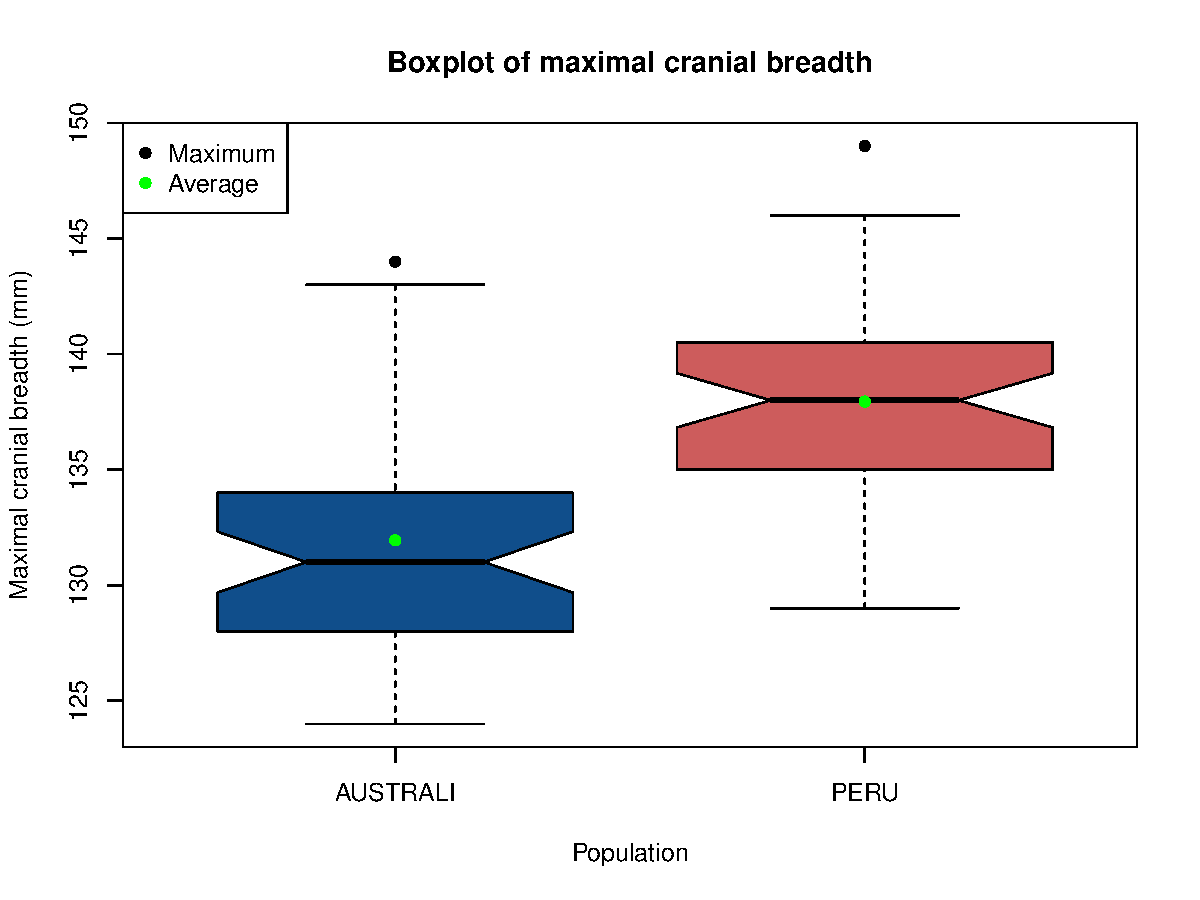
\includegraphics[width=.6\textheight,height=.45\textheight]{figure/unnamed-chunk-5-1} 

}

\caption[Boxplot of maximal cranial breadth(mm)]{Boxplot of maximal cranial breadth(mm)}\label{fig:unnamed-chunk-5}
\end{figure}
\end{Schunk}

\newpage
Created histogram of maximum cranial breadth for each population.

\begin{Schunk}
\begin{Sinput}
def.par <- par()
layout(matrix(c(1, 2), nrow=1, ncol=2), widths=c(0.5, 0.5))
#layout.show(n=2)
hist(
  xcb.australi, 
  main = "Australi population", 
  xlab = "Maximal cranial breadth(mm)", 
  ylab = "Count", 
  col = australi.peru.cols[1]
)
hist(
  xcb.peru, 
  main = "Peru population", 
  xlab = "Maximal cranial breadth(mm)", 
  ylab = "Count", 
  col = australi.peru.cols[2]
)
\end{Sinput}
\begin{figure}[h]

{\centering 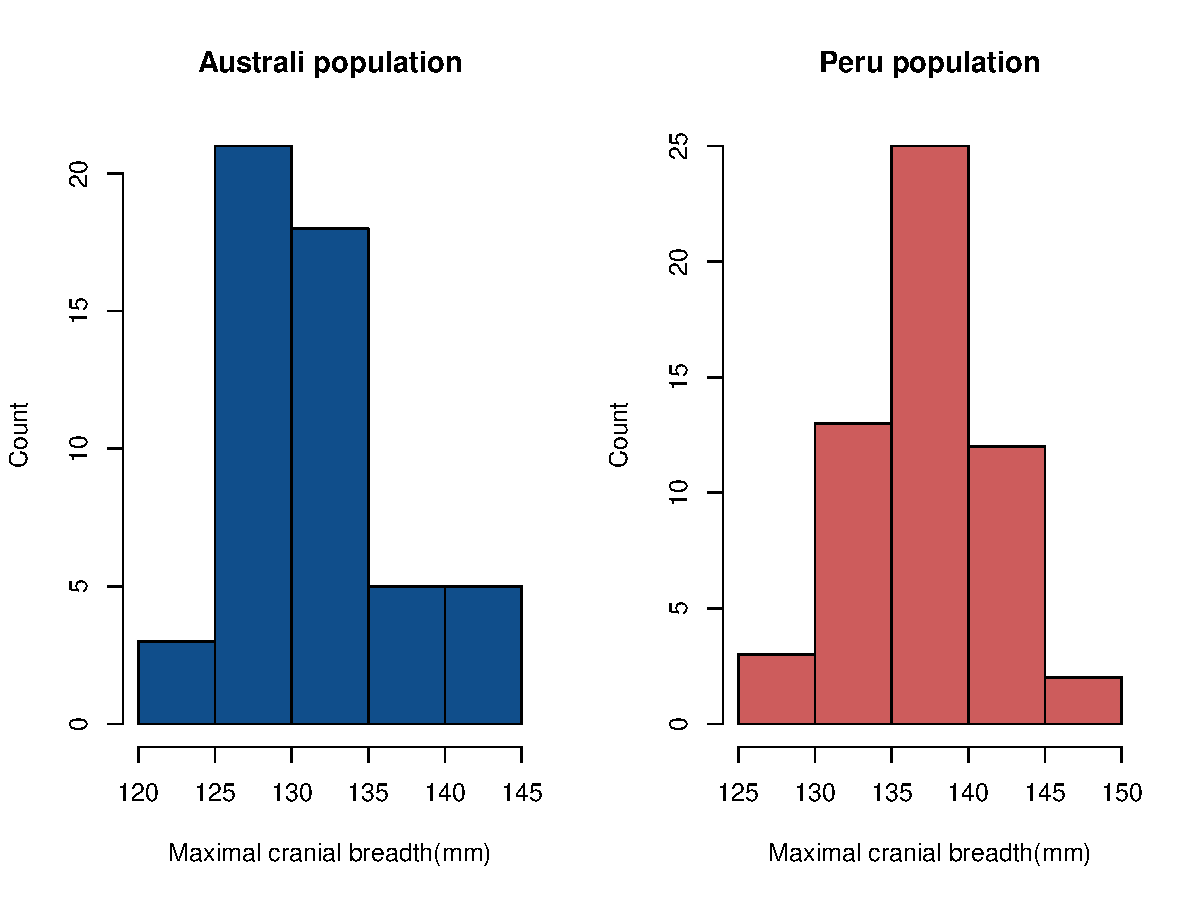
\includegraphics[width=.6\textheight,height=.45\textheight]{figure/unnamed-chunk-6-1} 

}

\caption[Histogram of maximal cranial breadth(mm)]{Histogram of maximal cranial breadth(mm)}\label{fig:unnamed-chunk-6}
\end{figure}
\end{Schunk}

\bigskip
\newpage
Created normal qq-plot of maximum cranial breadth for each population.

\noindent The observed measurements(Y axis values) are from the same range so the plots can be easily compared.

\begin{Schunk}
\begin{Sinput}
layout(matrix(c(1, 2), nrow=1, ncol=2), widths=c(0.5, 0.5))
#layout.show(n=2)
qqnorm(
  y = xcb.australi, 
  main = "Australi population", 
  xlab = "Theoretical quantities", 
  ylab = "Maximal cranial breadth(mm)",
  ylim = c(min(xcb.australi, xcb.peru), max(xcb.australi, xcb.peru)),
  pch = 16,
  col = australi.peru.cols[1]
)
qqline(xcb.australi)
qqnorm(
  y = xcb.peru, 
  main = "Peru population", 
  xlab = "Theoretical quantities", 
  ylab = "Maximal cranial breadth(mm)",
  ylim = c(min(xcb.australi, xcb.peru), max(xcb.australi, xcb.peru)),
  pch = 16,
  col = australi.peru.cols[2]
)
qqline(xcb.peru)
\end{Sinput}
\begin{figure}[h]

{\centering 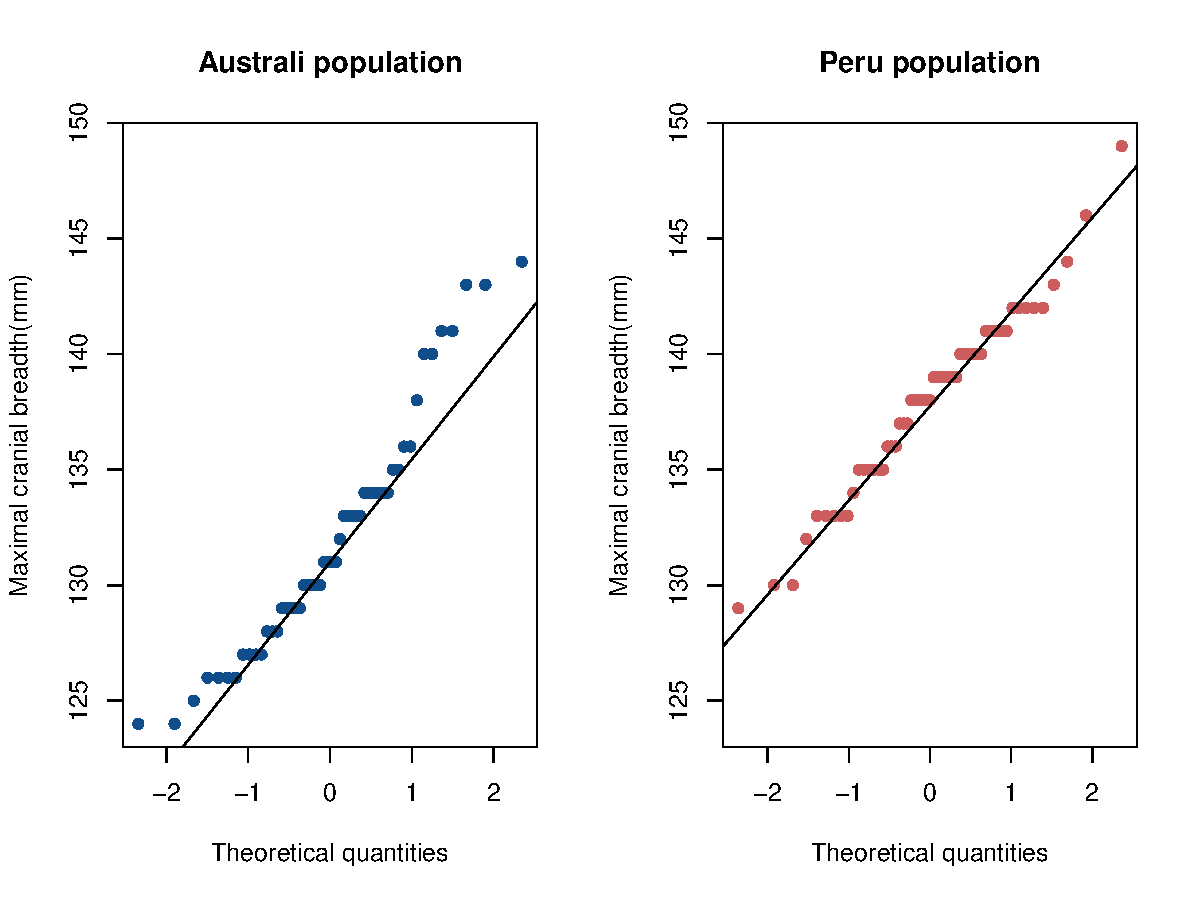
\includegraphics[width=.6\textheight,height=.45\textheight]{figure/unnamed-chunk-7-1} 

}

\caption[Normal qq-plot of maximal cranial breadth(mm)]{Normal qq-plot of maximal cranial breadth(mm)}\label{fig:unnamed-chunk-7}
\end{figure}
\end{Schunk}

\newpage
\subsection*{Results and interpretation}

Although both populations have same maximal cranial breadth reached, the differences can be best seen in histograms - more people of 
Peru population have bigger breadth than Australian people. 

Variable XCB, representing maximal cranial breadth of each population, 
seems to be normally distributed variable in both cases.

\newpage
\section*{Exercise 2}

First, I loaded the data. Then I checked for missing values in desired subset. There were none. So I summed the values in each column, which gave me a total sum of men and women in each year. Lastly, I added margins, which gave me total population in all of the years.
Also, I like to keep variables at the beggining of each significant part, in this case Exercise.

\begin{Schunk}
\begin{Sinput}
area.esp <- read.csv("area_spanish_provinces.csv", header = TRUE)
pop.esp <- read.csv2("population-spain-1998-2018.csv", header = TRUE)
#str(area.esp)
#str(pop.esp)
#pop.esp
#sum(is.na(pop.esp[, 2:length(pop.esp)])) = 0
### VARIABLES ###
legend.sex <- c("Women", "Men")
stat.years <-  c("1998", "2018")
total.pop.cols = c("pink", "dodgerblue")
year.cols = c("darkgoldenrod", "chocolate")
### VARIABLES ###
people.each.year <- as.table(colSums(pop.esp[, 2:length(pop.esp)]))
total.people.each.year <- addmargins(people.each.year, FUN = c(Total=sum))
\end{Sinput}
\end{Schunk}

Then I created a barplot of total population of Spain in each of the years, with each bar divided between men and women. 

\noindent The data were stored as table(from previous task), so I converted them into data frame to be able to subset values. 

\noindent The years were descending from 2018, so I made them ascending. 

\noindent Then I stored the data in matrix in order for barplot to accept the argument type. Since the data in data frame is ordered by gender, I simply added "byrow = TRUE" to the matrix in order to store the data correctly. 

\noindent I have also set a few plot parameters: 

"cex.axis", to make Y axis values smaller,

"las", to make axis labels horizontal,

"bty" in legend to hide legend box.

\begin{Schunk}
\begin{Sinput}
df.people <- as.data.frame(people.each.year)
# switched ordering of years
df.people <- df.people[dim(df.people)[1]:1, ]
df.people <- matrix(
  df.people[, 2], 
  nrow = 2, 
  ncol = 5,
  byrow = TRUE,
  dimnames = list(c("F", "M"), c("1998", "2003", "2008", "2013", "2018"))
)
# It is clean now
suppressWarnings(par(def.par))
barplot(
  height = df.people, 
  main = "Total population of Spain", 
  ylim = c(0, max(df.people)), 
  beside = TRUE, 
  las = 1,
  cex.axis = 0.8,
  col = total.pop.cols
)
legend('topleft', pch = 15, legend = legend.sex, col = total.pop.cols, bty = 'n')
\end{Sinput}
\begin{figure}[h]

{\centering 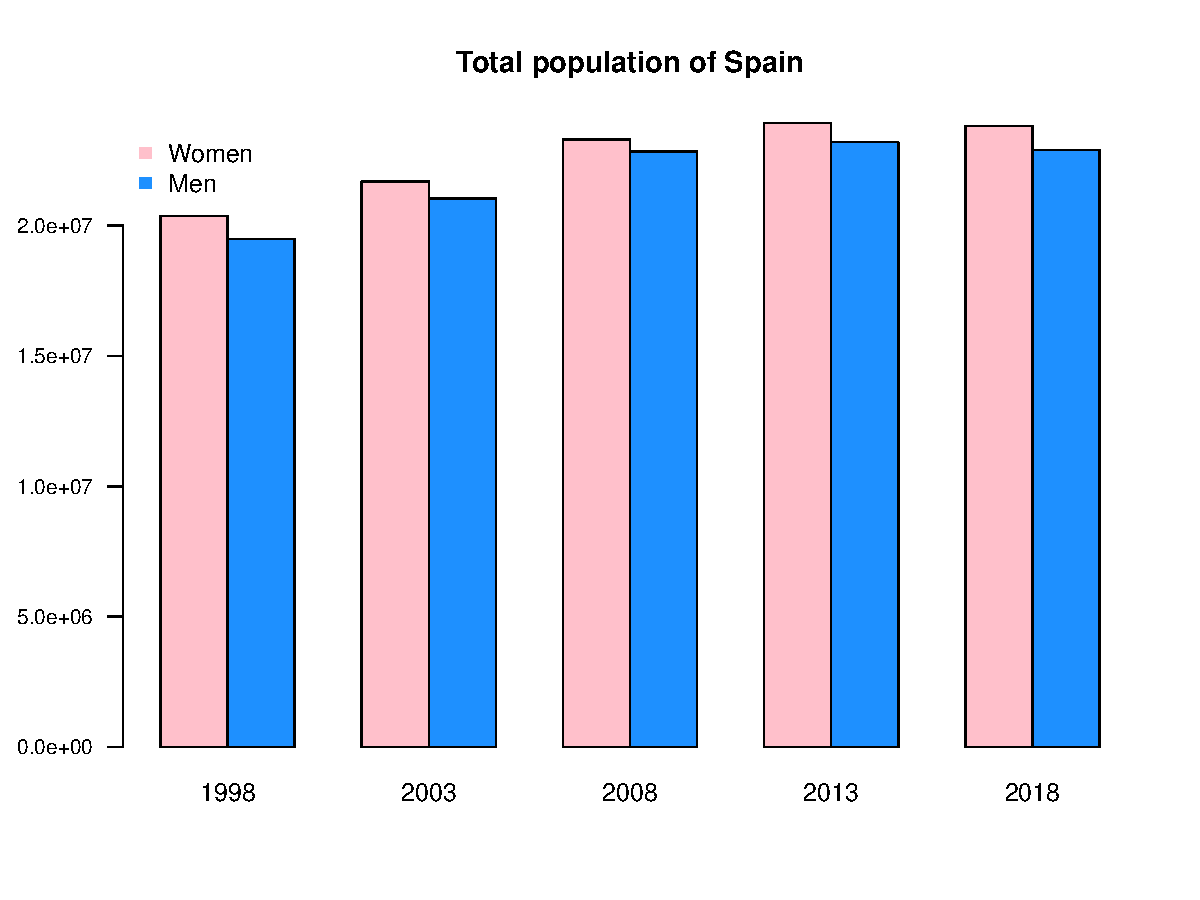
\includegraphics[width=.6\textheight,height=.45\textheight]{figure/unnamed-chunk-9-1} 

}

\caption[Barplot of total population in Spain]{Barplot of total population in Spain}\label{fig:unnamed-chunk-9}
\end{figure}
\end{Schunk}

\newpage
Then I created a barplot of relative proportions of men and women in each province in 2018. 

\noindent I transposed the input matrix in order to show the data by row(men and women side-by-side). I have also set few plot parameters: 

"cex.names", to make the provinces' names smaller, 

"las", to make axis labels perpendicular to the axis.

\begin{Schunk}
\begin{Sinput}
relative.pop.2018.provinces <- matrix(
  data = c(pop.esp$females.2018, pop.esp$males.2018),
  nrow = 52,
  ncol = 2
)
barplot(
  height = t(relative.pop.2018.provinces), 
  names.arg = pop.esp$province, 
  cex.names = 0.6, 
  cex.axis = 0.8, 
  main = "2018 relative population of Spain", 
  ylim = c(0, max(relative.pop.2018.provinces)), 
  las = 2, 
  beside = TRUE, 
  col = total.pop.cols
)
legend('topleft', pch = 15, legend = legend.sex, col = total.pop.cols, bty = 'n')
\end{Sinput}
\begin{figure}[h]

{\centering 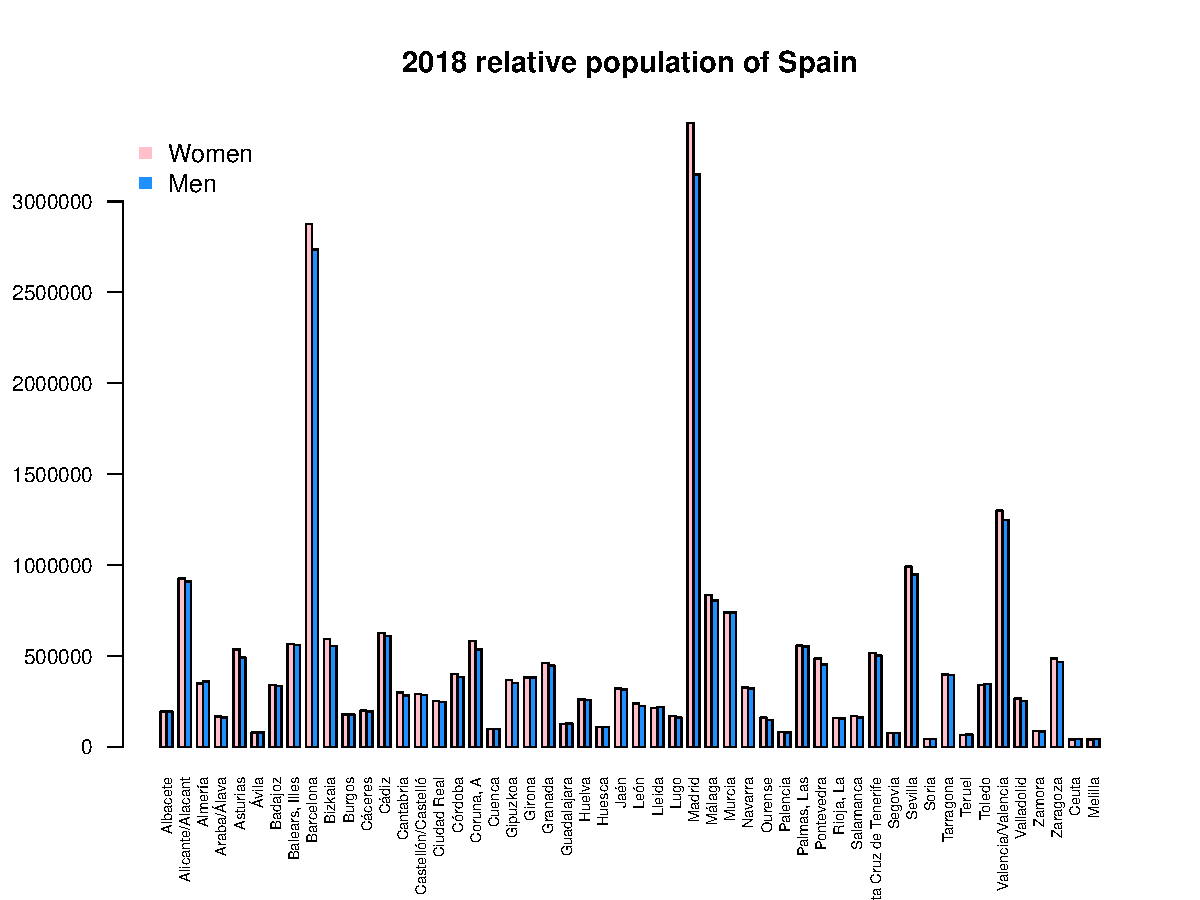
\includegraphics[width=.6\textheight,height=.45\textheight]{figure/unnamed-chunk-10-1} 

}

\caption[Barplot of relative population of Spain in 2018]{Barplot of relative population of Spain in 2018}\label{fig:unnamed-chunk-10}
\end{figure}
\end{Schunk}

\newpage
Then I calculated population density in 1998 and 2018, for each province. The are of each province was loaded in the beginning of this exercise. I created a helper matrix to store intermediate values.

\begin{Schunk}
\begin{Sinput}
ppl.in.two.years <- matrix(
  data = c(
    pop.esp$males.1998,
    pop.esp$females.1998,
    pop.esp$males.2018,
    pop.esp$females.2018
    ),
  nrow = nrow(pop.esp),
  ncol = 4,
  dimnames = list(pop.esp$province, c("males.1998", "females.1998", "males.2018", "females.2018"))
)
total.1998 <- as.vector(rowSums(ppl.in.two.years[, 1:2]))
total.2018 <- as.vector(rowSums(ppl.in.two.years[, 3:4]))
density.1998 <- total.1998 / area.esp$Area
density.2018 <- total.2018 / area.esp$Area
den <- data.frame(
  Province=pop.esp$province,
  "Year 1998" = density.1998, 
  "Year 2018" = density.2018
)
\end{Sinput}
\end{Schunk}

\noindent In subtask a, fistly, I sorted the data by year. Next, I calculated the estimates of characteristics of population density, each year separately. Lastly, I bound them together into one table.

\begin{Schunk}
\begin{Sinput}
# subtask a)
den.sorted.1998 <- sort(den$Year.1998)
den.sorted.1998.tab <- round(data.frame(
  size=length(den.sorted.1998),
  mean=MySampleMean(den.sorted.1998), 
  MyFiveNumSum(den.sorted.1998),
  skew=MySampleSkewCramer(den.sorted.1998), 
  kurt=MySampleKurtosis(den.sorted.1998),
  sd=MySampleSd(den.sorted.1998)
), 4)
den.sorted.2018 <- sort(den$Year.2018)
den.sorted.2018.tab <- round(data.frame(
  size=length(den.sorted.2018),
  mean=MySampleMean(den.sorted.2018), 
  MyFiveNumSum(den.sorted.2018),
  skew=MySampleSkewCramer(den.sorted.2018), 
  kurt=MySampleKurtosis(den.sorted.2018),
  sd=MySampleSd(den.sorted.2018)
), 4)
density.characteristics <- rbind(den.sorted.1998.tab, den.sorted.2018.tab)
row.names(density.characteristics) <- stat.years
\end{Sinput}
\end{Schunk}
% latex table generated in R 3.6.3 by xtable 1.8-4 package
% Fri Apr 10 11:54:41 2020
\begin{table}[ht]
\centering
\begin{tabular}{rrrrrrrrrrr}
  \hline
 & size & mean & min & lower.q & median & upper.q & max & skew & kurt & sd \\ 
  \hline
1998 & 52.00 & 282.01 & 9.17 & 29.36 & 79.29 & 118.94 & 4623.69 & 4.12 & 16.24 & 848.58 \\ 
  2018 & 52.00 & 356.87 & 9.02 & 28.23 & 84.74 & 151.19 & 6644.92 & 4.38 & 19.20 & 1128.98 \\ 
   \hline
\end{tabular}
\caption{Characteristics of population density of Spain in 1998 and 2018} 
\end{table}


\noindent In subtask b, I created a boxplot of population density in 1998 and in 2018. I have set the Y axis limits in order to see the graphs nicely, because there were some outliers which would squish the whole plot.

\begin{Schunk}
\begin{Sinput}
# subtask b)
suppressWarnings(par(def.par))
boxplot(
  den[2:3],
  notch = TRUE,
  main = "Pop. density in 1998 & 2018",
  ylab = "Population density",
  ylim = c(0, 250),
  pch = 16,
  col = year.cols
)
\end{Sinput}
\begin{figure}[h]

{\centering 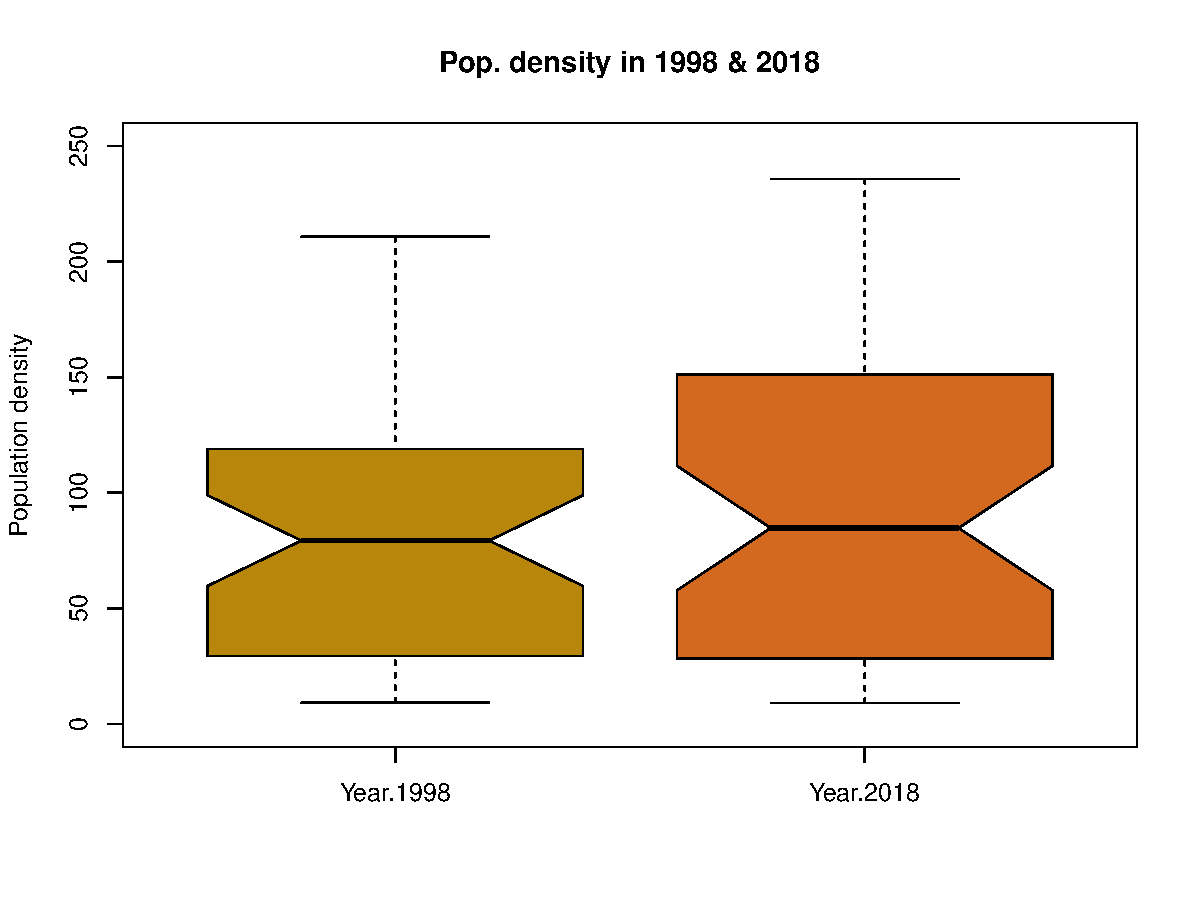
\includegraphics[width=.6\textheight,height=.45\textheight]{figure/unnamed-chunk-13-1} 

}

\caption[Boxplot of population density in Spain in 1998 and 2018]{Boxplot of population density in Spain in 1998 and 2018}\label{fig:unnamed-chunk-13}
\end{figure}
\end{Schunk}

\newpage
\noindet In subtask c, I created histogram of population density in 1998 and in 2018. There are two histograms, one for each year. Histogram for year 2018 is overlapping histogram for year 1998.

I changed the number of breaks. I was hoping to achieve a plot with province names, just like barplot of relative population of Spain(Figure 5), but it did not turn out that way. I'm really sad because that would make comparisons far better. Now I can't recognize the provinces.
I left it as it is because I still think it looks better than the default.

Lastly, I also changed axes a little bit because I didn't like the values inserted by default, they were too sparse, too spread out. 

\begin{Schunk}
\begin{Sinput}
# subtask c)
suppressWarnings(par(def.par))
rgb.cols = c(rgb(0.6,0.4,0.2,0.5), rgb(0.3,0.5,0.6,0.5))
hist(
  den$Year.1998, 
  main = "Pop. density in 1998 & 2018", 
  xlab = "Density(people/km^2)", 
  ylab = "Number of provinces", 
  las = 2, 
  col = rgb.cols[1], 
  breaks = density.characteristics$size[1], 
  xaxt = 'n', 
  yaxt = 'n'
)
# X axis
axis(
  side = 1, 
  at = seq(0, max(density.characteristics$max), by = 250), 
  las = 2, 
  cex.axis = 0.8
)
# Y axis
axis(
  side = 2, 
  at = seq(0, density.characteristics$size[1], by = 5), 
  las = 2, 
  cex.axis = 0.8
)
hist(
  den$Year.2018, 
  col = rgb.cols[2], 
  breaks = density.characteristics$size[2], 
  add = T)
legend('topright', pch = 15, legend = stat.years, col = rgb.cols, bty = 'n')
\end{Sinput}
\begin{figure}[h]

{\centering 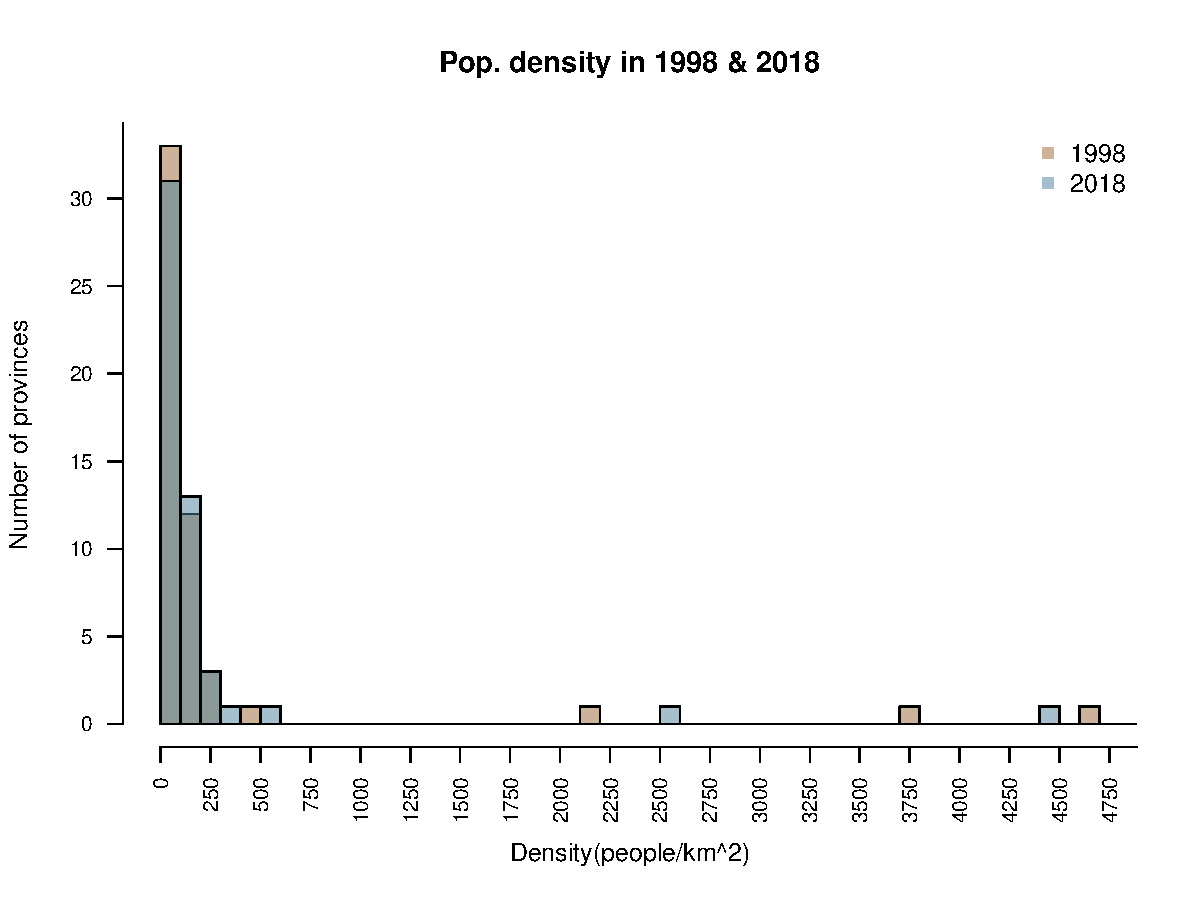
\includegraphics[width=.6\textheight,height=.45\textheight]{figure/unnamed-chunk-14-1} 

}

\caption[Histogram of population density in Spain in 1998 and 2018]{Histogram of population density in Spain in 1998 and 2018}\label{fig:unnamed-chunk-14}
\end{figure}
\end{Schunk}

\newpage
\subsection*{Results and interpretation}

Total population of Spain increased in years 1998-2018, even though there is a minor decrease between years 2013 and 2018.

Women are still slightly dominant when it comes to population proportions.

As we can see from the population density characteristics, the maximum population density increased from ~4600 to ~6600, which can also be seen in histogram. The mean population density increased from ~282 to ~356, which can be seen better e.g. in boxplot.

\end{document}
